\chapter{Approximate Bayesian Computation}
\label{chap:abc}

This chapter discusses the methodology of Approximate Bayesian Computation (ABC). We first motivate the use of ABC methods in our problem in \autoref{sec:abc-motivation}. Then, in \autoref{sec:abc-general}, we describe the method in general and discuss some limitations. \autoref{sec:abc-ssm} then introduces the ABC to our state-space model framework, and addresses some potential issues through kernel functions. Finally, in \autoref{sec:abcmh}, we summarize how exactly is the ABC method used in our model, and provide an alternative variant of the Metropolis-Hastings algorithm which relies on ABC instead of the particle filter to estimate the likelihood.


\section{Motivation} \label{sec:abc-motivation}
In the previous chapter, we have derived a way to bypass the likelihood function evaluation when calculating the Metropolis-Hastings acceptance ratio. The method relies on the particle filter to calculate a set of weights $w_t^{(i)} \propto \obs_t(\by_t \mid \bx_t^{(i)}, \btheta)$, where $\obs_t$ is the observation model defined in \eqref{eq:factorization}. These weights are then used to estimate the likelihood $p(\by_{1:T} \mid \btheta)$, as given in \eqref{eq:likelihood-estimate}. However, calculating the weights in such way requires full knowledge of this observation model.

In practice, one may not have access to a correct observation model in the form of a probability density $\obs_t$. Instead, only a model of the process which generates an observation $\by_t$ from the latent state $\bx_t$ may be available. This generative process may take the form of a differential equation, chemical reaction, simulation, etc. One is then in possession of a mean to generate an observation, but not to evaluate how probable it is. By attempting to fit an arbitrary probability distribution to this generative model, an error is necessarily introduced. The particle filter weights might then not reflect reality, and would lead to incorrect results when using such misspecified model for $\obs_t$.

Instead, we can utilize our knowledge of the generative process $\bx_t \mapsto \by_t$ to simulate a number of pseudo-observations $\bu_t$, and use them to approximate the likelihood ${p(\by_{1:T} \mid \btheta)}$. Then, we need not evaluate $\obs_t$, and so inference can proceed even without knowing the observation model density. This is exactly the idea behind the approximate Bayesian computation methodology, and is discussed in more detail in the next section.

Unfortunately, such approximation comes with a price. In \autoref{chap:inference}, it has been shown that using the particle filter does not introduce any approximation error, since the likelihood estimate is unbiased, and leaves the limiting distribution of the Metropolis-Hastings Markov chain intact. This is not the case when applying ABC methods, and is addressed in \autoref{sec:abc-ssm}.


\section{ABC in general} \label{sec:abc-general}
Before describing how to apply ABC in our SSM framework in \autoref{sec:abc-ssm}, we first review the method in general. Since the SSM framework does not require as general variant, we do not give a detailed treatment, and instead refer the reader to some of the literature mentioned below. This section should mostly give an idea of what exactly does ABC attempt to accomplish. Later on, we spend more time discussing the parts relevant to our problem.

One thing to note is that ABC has traditionally been applied to estimate the posterior $p(\btheta \mid \by)$ for some parameter $\btheta$ and observation $\by$. The method is considered with this in mind, and in \autoref{sec:abc-ssm}, we describe how use it to estimate the likelihood instead.

\paragraph{Approximate Bayesian Computation}
The methodology of ABC dates back to \cite{abc-old-old}, where a procedure using simulated psedudo-observations to approximate the posterior distribution was first described. Lately, ABC methods have gained popularity in modelling biological processes \citep{abc-old}. A more recent review can be found in \cite{abc-recent}.

In its classical formulation, ABC provides a way to approximate an intractable posterior ${p(\btheta \mid \by) \propto p(\by \mid \btheta) \pprior(\btheta)}$ by introducing an auxiliary variable $\bu$. The posterior approximation is then constructed by integrating over this variable \citep{jasra-filtering}, and considering only values sufficiently close to the true measurement. It takes the form of
\begin{equation} \label{eq:abc-integral}
p(\btheta \mid \by) \approx p^\epsilon(\btheta \mid \by) = \frac{\int \I_{\A_{\epsilon, \by}}(\bu) p(\bu \mid \btheta) \pprior(\btheta) \; \dx{\bu}}{\int_{\A_{\epsilon, \by}} \dx{\bu}},
\end{equation}
where $\I_{\A_{\epsilon, \by}}$ is the indicator function of a set $\A_{\epsilon, \by} = \left\{\bu \in \R^{d_y} : \rho(\bu, \by) \leq \epsilon \right\}$ and ${\rho: \R^{d_y} \times \R^{d_y} \to \R}$ is a metric, typically the Euclidean distance.

The motivation behind \eqref{eq:abc-integral} is that such integral can be approximated by randomly sampling from the likelihood $p(\cdot \mid \btheta)$ without needing to evaluate it. This way, the likelihood can exist only conceptually, and we are able to simulate samples $\bu$ from a model reflecting some real-world process, without considering the underlying probability density.

The hyper-parameter $\epsilon \geq 0$ controls how far can the auxiliary variable $\bu$ be from the true measurement $\by$ for them to be considered similar. Clearly, if we set $\epsilon = 0$, the integral becomes $p(\by \mid \btheta) \pprior(\btheta)$, and we recover the true posterior. In general, the smaller $\epsilon$, the better approximation is obtained, though at the cost of increased computational complexity, discussed in the next paragraph.

To avoid the curse of dimensionality, a summary statistic $\bm{s}: \R^{d_y} \to \R^p$, $1 \leq p < d_y$ is often introduced. Instead of comparing $\rho(\bu, \by) \leq \epsilon$, one then compares $\rho(\bm{s}(\bu), \bm{s}(\by)) \leq \epsilon$ (assuming that the metric has been redefined to $\rho: \R^p \times \R^p \to \R$).

It can be shown that if $\bm{s}$ is a sufficient statistic for the parameter $\btheta$, the probability density $p^\epsilon(\btheta \mid \by)$ converges to $p(\btheta \mid \by)$ as $\epsilon \to 0$ \citep{jasra-time-series}. However, it is typically impossible to find such statistic outside of the exponential family of distributions. Otherwise, using a statistic that is not sufficient introduces an additional approximation error.

\paragraph{Basic version of the ABC simulation}
We now give a basic variant of a sampling-based approximation to $p^\epsilon(\btheta \mid \by)$. In the spirit of \eqref{eq:abc-integral}, the algorithm performs rejection sampling by comparing whether a sampled $\bu$ is in $\A_{\epsilon, \by}$ or not. After describing the algorithm, we discuss some limitations of this basic approach.
\begin{algorithm}[ht]
    \caption{ABC Rejection Algorithm}
    \label{alg:abc-rejection}
    \begin{algorithmic}[1]
        \Input $\text{Number of samples } M, \text{ observation } \by, \text{ metric } \rho, \text{ maximum distance } \epsilon.$
        
        \State $i \gets 1$
        
        \While{$i \leq M$}
        \State $\text{Sample } \btheta^\prime \sim \pprior(\cdot).$ \Comment{Sample from the prior.}
        \State $\text{Simulate } \bu \text{ from } p(\cdot \mid \btheta^\prime).$ \Comment{Simulate a pseudo-observation.}
        
        \If {$\rho(\bu, \by) \leq \epsilon$}
        \State $\btheta^{(i)} \gets \btheta^\prime$ \Comment{Accept the proposed sample.}
        \State $i \gets i + 1$
        \EndIf
        \EndWhile
        
        \Output $\text{Accepted samples } \left\{ \btheta^{(1)}, \ldots, \btheta^{(M)} \right\}.$
    \end{algorithmic}
\end{algorithm}

The algorithm iteratively samples parameters $\btheta^\prime$ from the prior, plugs them into the likelihood $p(\cdot \mid \btheta^\prime)$, and simulates pseudo-observations $\bu$. These are then compared to the true measurement $\by$ using the metric $\rho$. If the proposed parameter $\btheta^\prime$ gave rise to a pseudo-observation similar enough to the true $\by$ (i.e. $\bu \in \A_{\epsilon, \by}$), the parameter is kept under the assumption that the true data are likely under $\btheta^\prime$. The ABC approximation is then given in terms of the accepted samples $\btheta^{(1)}, \ldots, \btheta^{(M)}$ as the empirical distribution
\begin{equation*}
p(\btheta \mid \by) \approx \frac{1}{M} \sum_{i=1}^M \delta_{\btheta^{(i)}}(\btheta).
\end{equation*}

Setting a low value of $\epsilon$ increases the approximation accuracy, at the cost of increased rejection rate. On the other hand, setting $\epsilon$ too large causes the algorithm to accept more often, but leads to simulating pseudo-measurements dissimilar to $\by$ and, in turn, incorrect $\btheta^{(i)}$. Setting a suitable value of $\epsilon$ is therefore the main difficulty when using ABC. Several approaches are discussed by \cite{jasra-filtering, jasra-time-series}. One particular way \citep{dedecius} is used in \autoref{sec:abc-ssm} in the context of SSMs.

There are many improvement to the basic ABC of \autoref{alg:abc-rejection}, discussed for instance by \cite{abc-recent}. In particular, more sophisticated sampling approaches relying again on MCMC are described. This is not an issue relevant to the SSM framework, as the samples are generated in a different fashion, given in the next section.

\section{ABC in SSMs} \label{sec:abc-ssm}
Next, we describe how exactly is the ABC methodology applied in the context of SSMs.

\autoref{sec:abc-general} states that the typical use case of ABC arises in cases where we have knowledge about the data-generating process, but are unable to evaluate the probability of such data. In the context of SSMs, this translates into knowing how the observed values $\by_t$ have been generated from the latent states $\bx_t$, but being unable to evaluate the density $\obs_t(\by_t \mid \bx_t, \btheta)$. This prevents us from calculating the importance weights $w_t$ through the particle filter, which relies on the availability of $\obs_t$.

The papers \cite{tina-toni} and \cite{jasra-filtering} describe how a filter could be constructed using the ABC approximation. Additionally, \cite{jasra-time-series} applies this filter in the context of SSMs. We first discuss the construction of this filter. Afterwards, we address a particular limitation of this approach through kernel functions.

\paragraph{Filter construction through ABC}
In SSMs, the observations $\by_t$ are typically low-dimensional, often scalar quantities. It is then not necessary to consider any summary statistics.

\cite{jasra-filtering} consider a modification of the particle filter (\autoref{alg:particle-filter}) which simulates pseudo-observations according to the observation model, and calculates the importance weights based on their closeness to the true measurements. The pseudocode is given in \autoref{alg:abc-filter}.

\begin{algorithm}[ht]
    \caption{ABC-based filter}
    \label{alg:abc-filter}
    \begin{algorithmic}[1]
        \Input $\text{Number of particles } N,\ \text{current parameter value } \btheta, \text{maximum distance } \epsilon,\ \left\{\by_1, \ldots, \by_T\right\}.$
        
        \State $\text{Sample } \bx_0^{(i)} \sim \sprior(\cdot \mid \btheta), \quad i = 1, \ldots, N.$ \Comment{Initialize $N$ particles.}
        
        \State $w_0^{(i)} \gets \frac{1}{N}, \quad i = 1, \ldots, N.$ \Comment{Initialize uniform weights.}
        
        \For{$t = 1\ \mathbf{to}\ T$}
        \State $\text{Sample } \bx_t^{(i)} \sim \trans_t(\bx_t \mid \bx_{t-1}^{(i)}, \btheta), \quad i = 1, \ldots, N.$ \Comment{Sample $N$ new particles.}
        
        \State $\text{Simulate } \bu_t^{(i)} \text{ from } \obs_t(\cdot \mid \bx_t^{(i)}), \quad i = 1, \ldots, N.$ \Comment{Simulate $N$ pseudo-observations.}
        
        \State $\text{Set } w_t^{(i)} \propto \I_{\A_{\epsilon, \by_t}}(\bu_t^{(i)}) w_{t-1}^{(i)}, \quad i = 1, \ldots, N.$
        
        \State $\text{Resample } \bx_t^{(i)} \text{ and reset } w_t^{(i)} \text{ using \autoref{alg:resampling}}, \quad i = 1, \ldots, N.$
        \EndFor
    \end{algorithmic}
\end{algorithm}

The algorithm proceeds similarly to \autoref{alg:particle-filter} except for the way the weights are computed. Instead of evaluating the unavailable density $\obs_t$ at the true observation $\by_t$, a pseudo-observation $\bu_t$ is simulated. The weight is then set to a non-zero value if ${\bu_t \in \A_{\epsilon, \by_t}}$, and 0 otherwise. It may seem that the weights for the same particle $i$ necessarily collapse to 0 after a number of time steps due to the recursive multiplication in step 6. However, step 7 resets the weights uniformly after resampling, so such collapse does not occur.

Analogously to \autoref{sec:particle-filter-estimate}, the weights are then used to approximate the likelihood $p(\by_{1:T} \mid \btheta)$. According to \cite{jasra-time-series}, the estimate is given by
\begin{equation} \label{eq:abc-likelihood}
\widehat{\aux} = \prod_{t=1}^T \frac{1}{N} \sum_{i=1}^N \frac{w_t^{(i)}}{\int_{\A_{\epsilon, \by_t}} \dx{\bu}}.
\end{equation}
The integral in the denominator essentially normalizes the weights $w_t^{(i)}$ to be equal to the probability density of $\mathcal{U}(\by_t; \epsilon)$, the uniform distribution in a sphere centered at $\by_t$ with radius $\epsilon$ given in terms of the metric $\rho$.

\paragraph{Bias}
The use of this ABC filter introduces bias to the parameter inference. Recall that in \autoref{sec:particle-filter-estimate}, we required $\widehat{\aux}$ to be an unbiased estimator of $p(\by_{1:T} \mid \btheta)$. This was the case when the weights were calculated according to $w_t^{(i)} \propto \obs_t(\by_t \mid \bx_t) w_{t-1}^{(i)}$. This unbiasedness is not preserved here, since $\widehat{\aux}$ estimates
\begin{equation*}
\begin{split}
p^\epsilon(\by_{1:T} \mid \btheta) &= \int p^\epsilon(\bx_{0:T}, \by_{1:T} \mid \btheta) \; \dx{\bx_{0:T}} \\
&= \int \sprior(\bx_0 \mid \btheta) \prod_{t=1}^T \trans_t(\bx_t \mid \bx_{t-1}, \btheta) \obs_t^\epsilon(\by_t \mid \bx_t, \btheta) \; \dx{\bx_{0:T}},
\end{split}
\end{equation*}
(compare the inside of the integral with \eqref{eq:factorization}), as noted by \cite{jasra-time-series}. Here the approximate observation density is given by the ABC form
\begin{equation*}
\obs_t^\epsilon(\by_t \mid \bx_t, \btheta) = \frac{\int \I_{\A_{\epsilon, \by_t}}(\bu) \obs_t(\bu \mid \bx_t, \btheta) \; \dx{\bu}}{\int_{\A_{\epsilon, \by_t}} \dx{\bu}},
\end{equation*}
similarly to \eqref{eq:abc-integral}. This essentially means that by plugging \eqref{eq:abc-likelihood} into the Metropolis-Hastings acceptance ratio, the limiting distribution of the underlying Markov chain becomes $p^\epsilon(\btheta \mid \by_{1:T}) \propto p^\epsilon(\by_{1:T} \mid \btheta) \pprior(\btheta)$, instead of the correct $p(\btheta \mid \by_{1:T})$. In general, this bias cannot be dealt with, and is a price to pay for using the incorrect observation model.

An interesting way to address this deficiency has been proposed by \cite{noisy-abc1} and by \cite{noisy-abc2}. The authors note that one uses data $\by_{1:T}$ assumed to have been generated according to \eqref{eq:factorization}, $p(\by_{1:T} \mid \btheta)$, but fitting the ABC approximation $p^\epsilon(\by_{1:T} \mid \btheta)$. In an attempt to bring the data closer the model being really fitted, the authors use a sequence of perturbed observations $\bm{z}_t = \by_t + \bm{v}$, $\bm{v} \sim \mathcal{U}(\bm{0}; \epsilon)$ which denotes the uniform distribution in a sphere given by $\rho$, with radius $\epsilon$ and centered at the origin. It is proved that if $\btheta$ is estimated according to maximum likelihood, the estimate is consistent when using the perturbed sequence $\bm{z}_{1:T}$. This approach is called the Noisy ABC.


\paragraph{Use of kernel functions}
A limitation of \autoref{alg:abc-rejection} and \autoref{alg:abc-filter} lies in the use of the indicator function $\I_{\A_{\epsilon, \by}}$. There are two problems:
\begin{enumerate}
    \item A practical one; it may happen that no samples are accepted, and the output is null in case of \autoref{alg:abc-rejection}, or too many weights become zero in case of \autoref{alg:abc-filter}, and the filter collapses.
    \item A more fundamental one, the simulated pseudo-observations $\bu_t$ are all assigned equal weights, regardless of how far they lie from the true measurement $\by_t$. Intuitively, a pseudo-observation closer to the true $\by_t$ should be assigned a higher weight than one which is further away.
\end{enumerate}
Both issues can be mitigated by considering a general kernel function in place of the indicator $\I_{\A_{\epsilon, \by}}$. Let a kernel of width $\epsilon$ centered at $\by$ and evaluated at $\bu$ be denoted by $\kappa(\bu; \by, \epsilon)$. In machine learning, kernel functions are often taken \emph{proportional} to some symmetric probability density function \citep{elements}. However, as we aim to replace the indicator function $\I_{\A_{\epsilon, \by}}$ by such kernel, we require the kernel to be properly normalized (integrate to unity), to mirror the normalization in \eqref{eq:abc-likelihood}.

With such kernel function, we can then write $w_t^{(i)} \propto \kappa(\bu_t; \by_t, \epsilon) w_{t-1}^{(i)}$. The likelihood estimate \eqref{eq:abc-likelihood} then becomes
\begin{equation} \label{eq:abc-likelihood-kernel}
\widehat{\aux} = \prod_{t=1}^T \frac{1}{N} \sum_{i=1}^N w_t^{(i)}
\end{equation}
due to the kernel having been normalized. This way, the weights are no longer uniformly set, but instead reflect the distance of $\bu_t$ from $\by_t$. There is also no risk of the filter collapsing due to majority of the weights becoming zero.

Introducing the kernel function to the weights computation is in principle similar to using importance sampling rather than simple rejection sampling \citep{information-theory}. Instead of accepting/rejecting the generated samples based on whether they match some criterion, they are all accepted, and weighted according to \emph{how well} they match it.

With the kernel functions in mind, we describe a procedure for automatic tuning of the kernel width $\epsilon$, which has been ignored thus far. The adopted method has been derived in a one-dimensional setting, i.e. $\bu, \by \in \R$. We thus denote $\by$ by $y$ and $\bu$ by $u$, them being scalar quantities. When considering multivariate observations, the kernels are applied coordinate-wise (assuming independence between the components of $\by$ or $\bu$, respectively).

Before describing the kernel tuning procedure, we give several examples of commonly used kernel functions and comment on their usage. The kernels are shown in \autoref{fig:kernels}.
\begin{enumerate}
    \item \textbf{Gaussian kernel} The Gaussian kernel takes the form
    \begin{equation*}
    \kappa(u; y, \epsilon) = \frac{1}{\sqrt{2 \pi \epsilon^2}} \exp \left\{-\frac{\left(u - y\right)^2}{2 \epsilon^2}\right\}.
    \end{equation*}
    It is one of the most-commonly used kernel functions.
    \item \textbf{Cauchy  kernel} The Cauchy kernel takes the form
    \begin{equation*}
    \kappa(u; y, \epsilon) = \frac{1}{\pi \epsilon \left[ 1 + \left(\frac{u - y}{\epsilon}\right)^2 \right]}.
    \end{equation*}
    As opposed to the Gaussian distribution, the Cauchy distribution has heavier tails, and so it is suitable for situations with potential distant observations. This kernel typically assigns non-trivial probability even to distant pseudo-observations, and so the filter does not collapse even under outliers.
    
    \item \textbf{Uniform kernel} The uniform kernel takes the form
    \begin{equation*}
    \kappa(u; y, \epsilon) = \begin{cases}
    \frac{1}{2 \epsilon}, & y - \epsilon < u < y + \epsilon; \\
    0, & \text{otherwise}.
    \end{cases}
    \end{equation*}
    Using this kernel, we recover the standard ABC which accepts $u$ if $u \in \A_{\epsilon, y} = \left\{u : \left| u - y \right| < \epsilon \right\}$. If we are in a situation with multivariate observations $\by_t$ and apply the uniform kernel coordinate-wise, the set of accepted samples coincides with the standard ABC using $\rho(\bu, \by) = \max_{i=1}^{d_y} \left|u_i - y_i\right|$, the $L_\infty$ distance.
\end{enumerate}

\begin{figure}[ht]
    \centering
    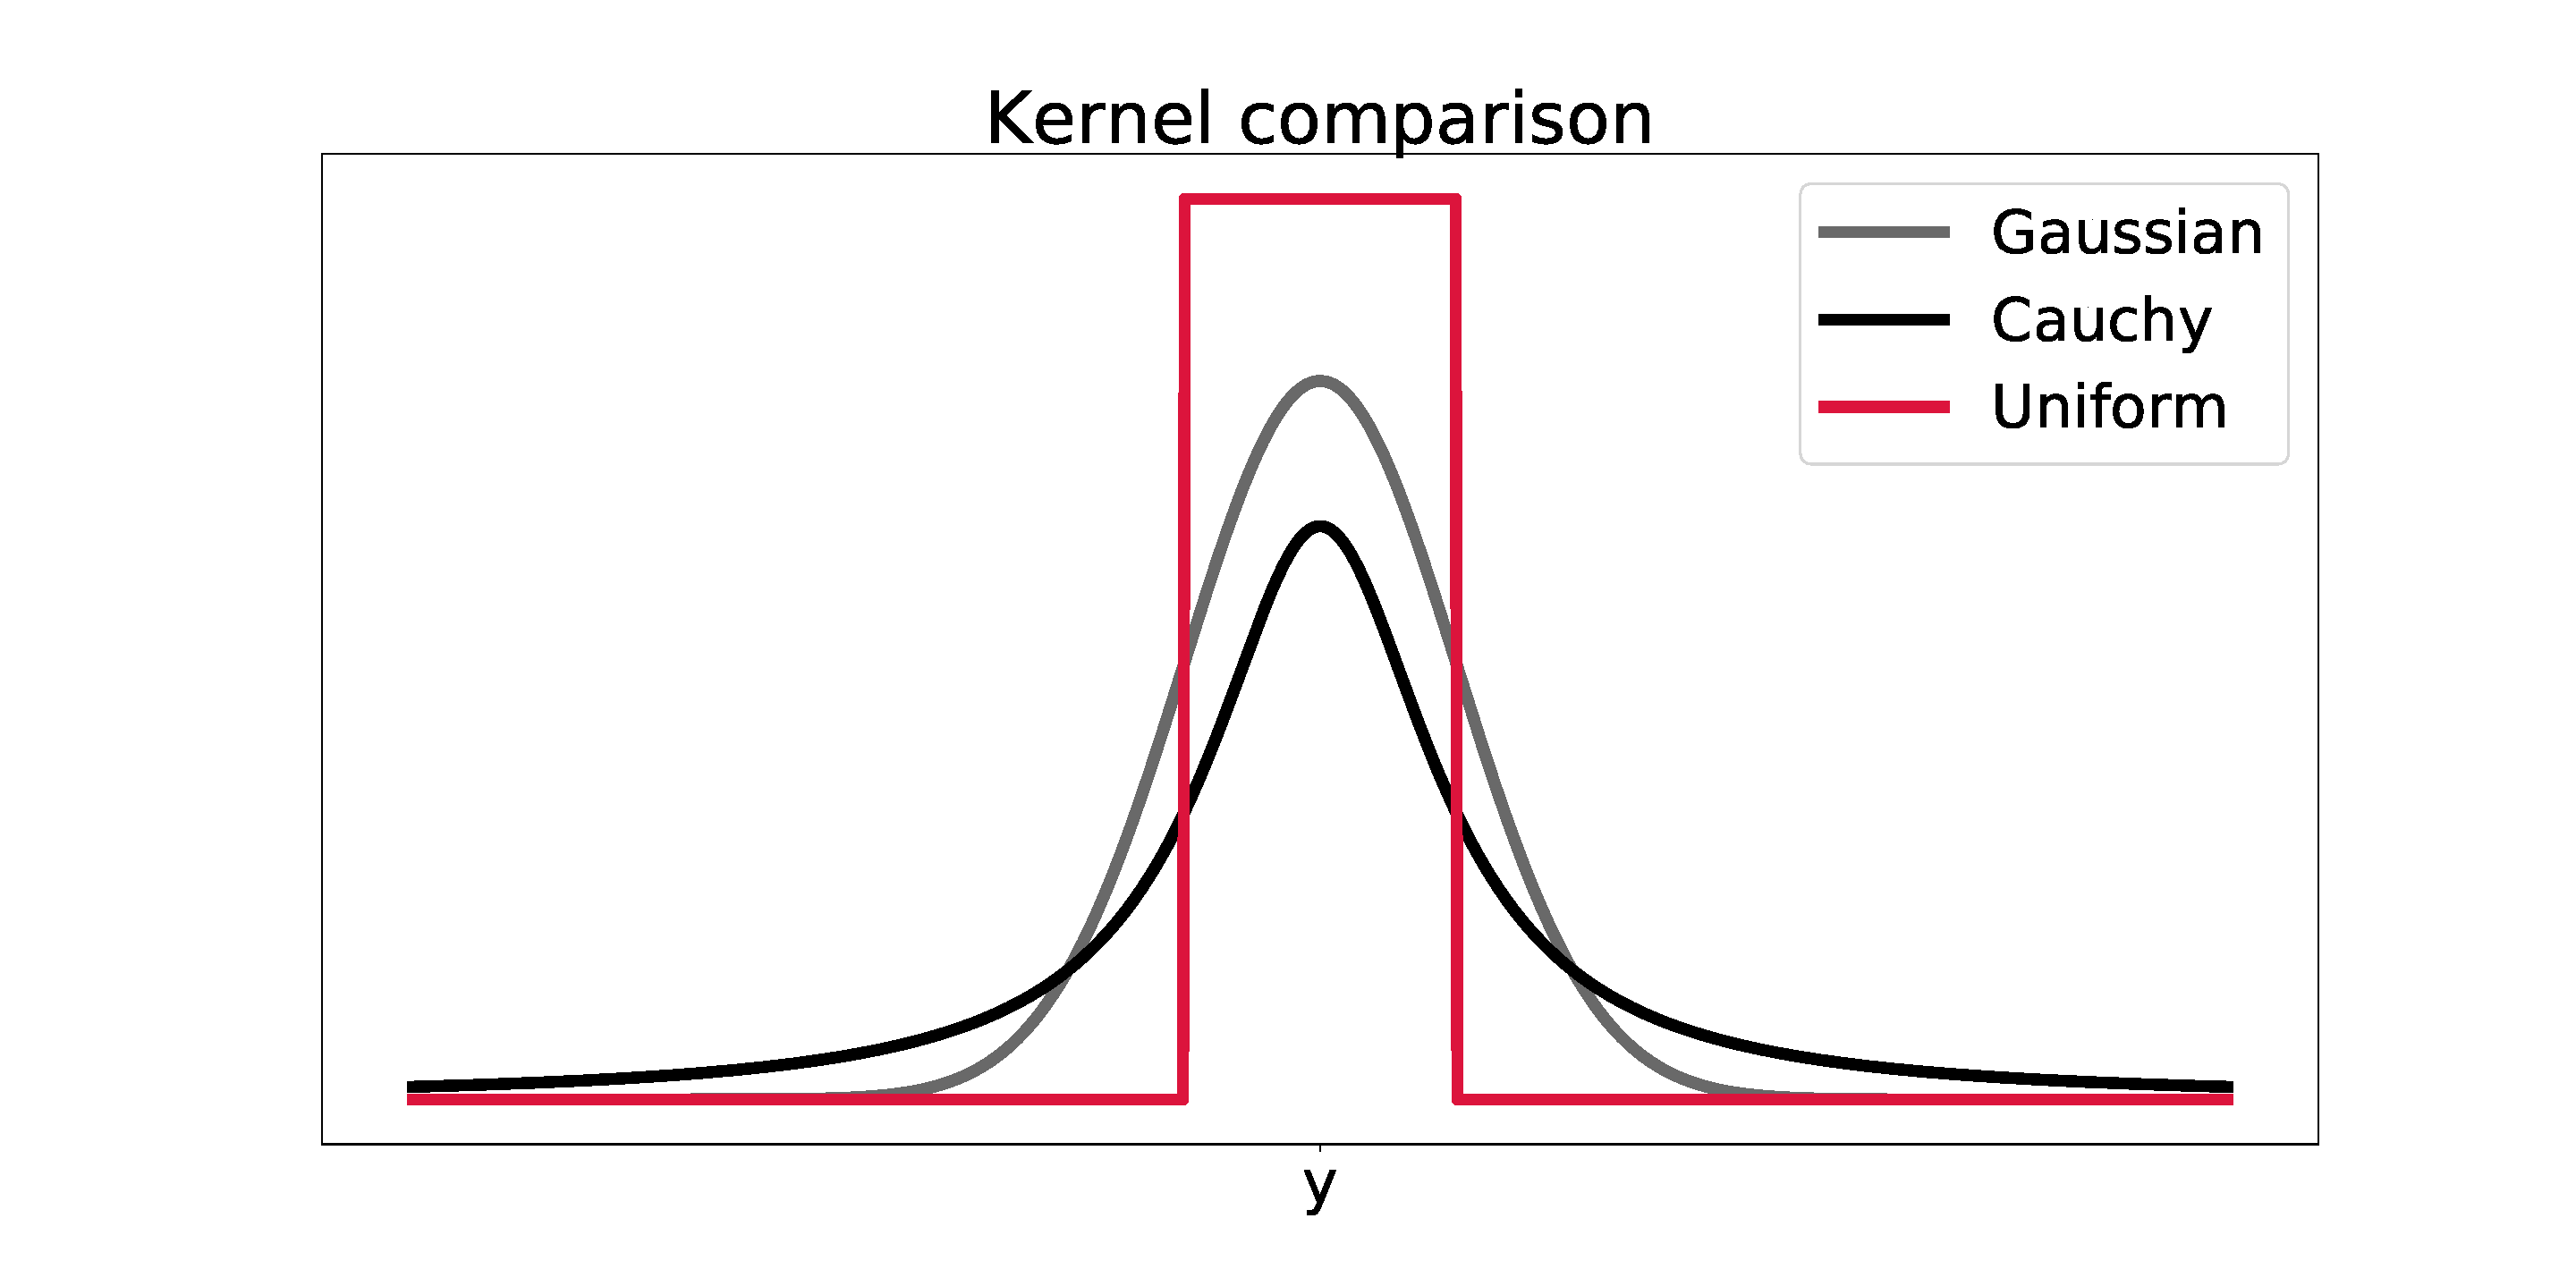
\includegraphics[width=\linewidth]{kernels}
    \caption{The Gaussian, Cauchy and uniform kernel functions centered at $y = 0$ with width $\epsilon = 3$.}
    \label{fig:kernels}
\end{figure}


The Noisy ABC procedure described above is then naturally generalized by perturbing the observations by samples from a given kernel, instead of the uniform distribution in a ball.


\paragraph{Kernel width tuning}
In this paragraph, we address the issue of tuning the kernel width $\epsilon$. Since the previous section has shown that the indicator function $\I_{\A_{\epsilon, \by}}$ is recovered by a particular kernel, the method also applies to the standard ABC formulation.

A careful setting of $\epsilon$ is necessary. When the kernel width is too low, most of the $N$ generated pseudo-observations are assigned with low probabilities, and the importance weights are close to zero. On the other hand, when the width is too high, even outlying pseudo-observations are assigned a non-trivial probability and shift the filter to incorrect values. In addition, the kernel becomes flat and close to the uniform variant. A manual setting of $\epsilon$ is thus a non-obvious task without any guidelines in the data. Additionally, the width should somehow reflect the filter evolution over time, since all observations $\by_t$ are different and may require different kernel widths.

In this thesis, we adopt a procedure described by \cite{dedecius}, which is briefly reviewed below. More details can be found in the original paper.

The method is based on the idea that the true observation model $\obs_t$ should cover a given number of generated pseudo-observations $\bu_t^{(i)}, i = 1, \ldots, N$ by a $100p\%$ high probability region ($p$-HPR), where $p \in \left(0, 1\right)$ is a given constant. If this is true, the pseudo-observations can be expected to describe the distribution $\obs_t$ sufficiently-well. As this distribution is not known, it is approximated by the kernel $\kappa$ evaluated at $\bu_t^{(i)}, i = 1, \ldots, N$.

As given in \eqref{eq:abc-likelihood-kernel}, the kernel is evaluated at each pseudo-observation $\bu_t^{(i)}, i = 1, \ldots, N$ while centered at $\by_t$. We then need to tune the width at time $t$, denoted $\epsilon_t$, so that a given fraction $\frac{\alpha}{N}$ of the pseudo-observations is covered by the $p$-HPR of the kernel. For the procedure to work, the kernel function $\kappa$ must be invariant under translation and scaling, i.e. belong to the location-scale family of distributions. Many popular kernels, including the three discussed above, belong to this family.

The tuning procedure involves two steps:
\begin{enumerate}
    \item Identify $u_t^{[\alpha]}$, the $\alpha$th closest pseudo-observation to $y_t$.
    \item Center the kernel $\kappa$ at $y_t$ and set the width $\epsilon_t$ so that
    \begin{equation} \label{eq:kernel-tuning-integral}
    \left| \int_{y_t}^{u_t^{[\alpha]}} \kappa(u_t; y_t, \epsilon_t) \; \dx{u_t} \right| = \frac{p}{2},
    \end{equation}
    meaning that $u_t^{[\alpha]}$ lies at the boundary of the $p$-HPR of $\kappa(\cdot; y_t, \epsilon_t)$.
\end{enumerate}
These two steps are visualized in \autoref{fig:kernel-tuning}. In case of multidimensional $\by_t$ and $\bu_t$, this procedure is performed coordinate-wise. 

\begin{figure}[ht]
    \centering
    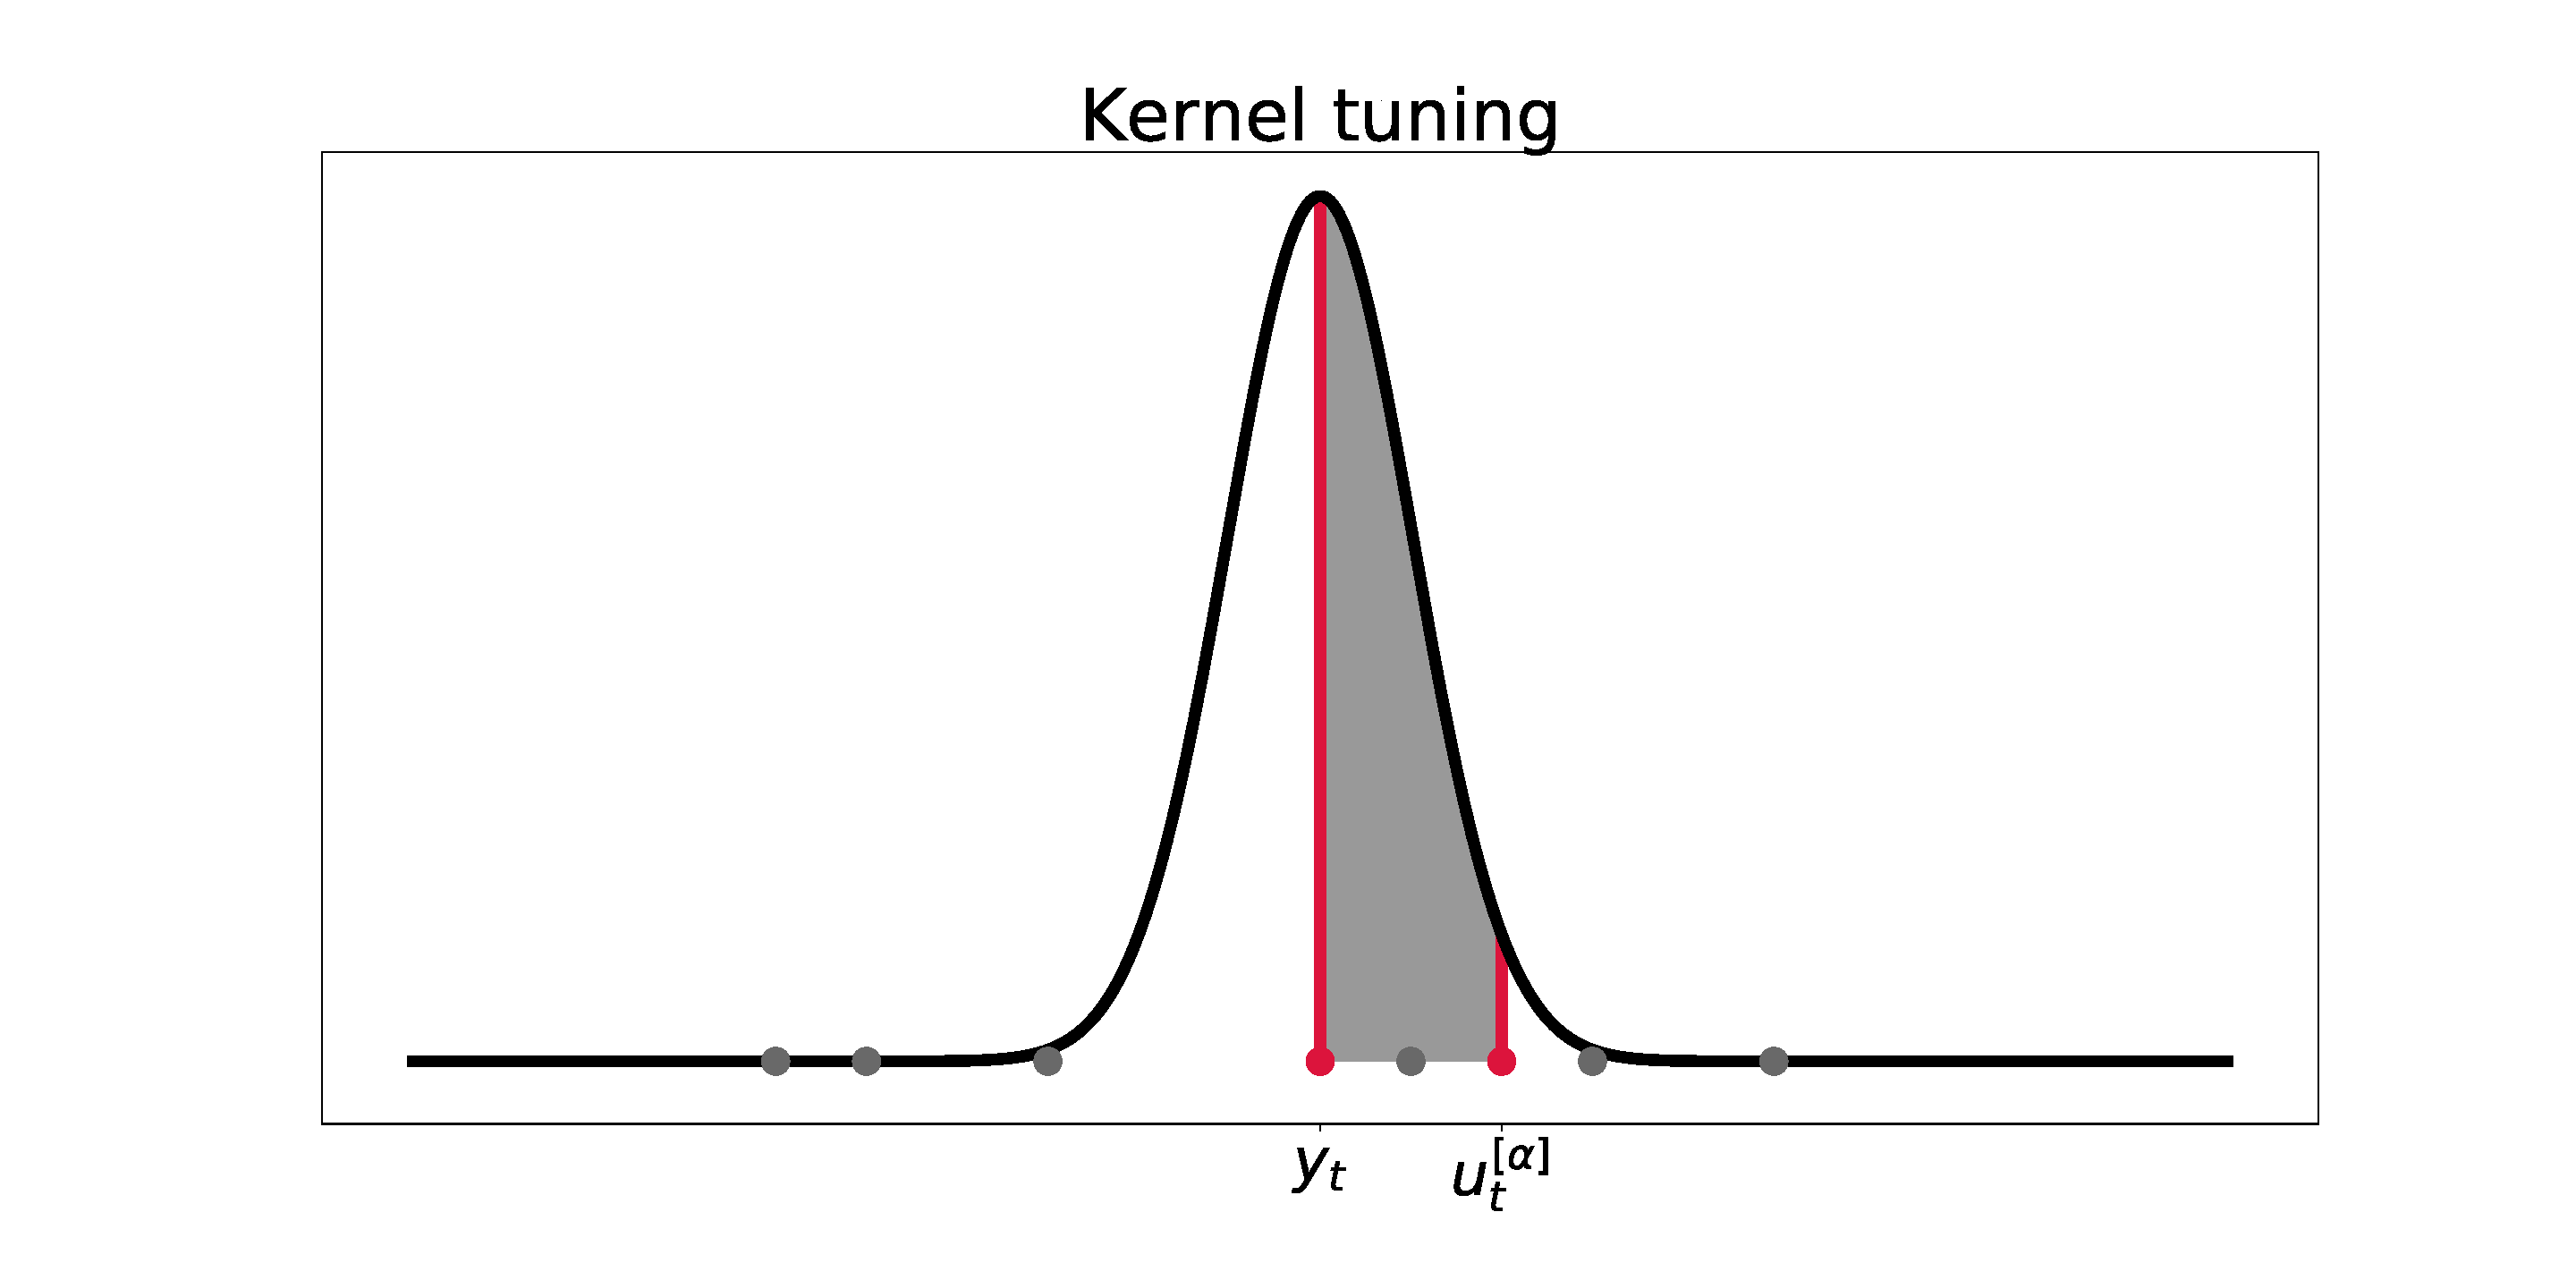
\includegraphics[width=\linewidth]{kernel_tuning}
    \caption{Visualization of the kernel tuning procedure. In this picture, ${\alpha = 2}$, ${p = 0.95}$, and the kernel is Gaussian. Plotted is the kernel along with a number of pseudo-observations $u_t^{(i)}$ and the true measurement $y_t$. Equation \eqref{eq:kernel-tuning-integral} states that the shaded area has volume $\frac{p}{2} = 0.475$.}
    \label{fig:kernel-tuning}
\end{figure}

The meaning of equation \eqref{eq:kernel-tuning-integral} is that $u_t^{[\alpha]}$ is either the $\frac{1-p}{2}$-quantile or the $\frac{1+p}{2}$-quantile of $\kappa(\cdot; y_t, \epsilon_t)$, depending on whether $u_t^{[\alpha]} \leq y_t$ or $u_t^{[\alpha]} \geq y_t$. If we restrict ourselves to symmetric kernels, we may get rid of this case division by exploiting kernel symmetry.

Let $F$ denote the cumulative distribution function of the kernel $\kappa(\cdot; 0, 1)$ centered at 0 with width $\epsilon = 1$. Let its quantile function be denoted by $F^{-1}$. From $\kappa$ belonging to the location-scale family, we get that the quantile function of a general kernel $\kappa(\cdot; y_t, \epsilon_t)$ is
\begin{equation} \label{eq:location-scale-quantile}
Q(\beta) = y_t + \epsilon_t F^{-1}(\beta), \quad \beta \in \left(0, 1\right).
\end{equation}
As \eqref{eq:kernel-tuning-integral} and the assumed kernel symmetry require $\left| u_t^{[\alpha]} \right|$ to be the $\frac{1+p}{2}$-quantile of $\kappa(\cdot; y_t, \epsilon_t)$, we can substitute $u_t^{[\alpha]}$ for $Q(\beta)$ in \eqref{eq:location-scale-quantile} and solve for $\epsilon_t$, obtaining
\begin{equation} \label{eq:kernel-tuning}
\epsilon_t = \frac{\left| u_t^{[\alpha]} - y_t \right|}{F^{-1}(\frac{1+p}{2})},
\end{equation}
where the absolute value comes from the kernel being symmetric, so it is irrelevant whether we consider pseudo-observations lower or greater than the true observation $y_t$. The quantile function $F^{-1}$ is uniquely associated with each kernel, and the only free parameters are $\alpha$ and $p$.


\section{Likelihood estimate through ABC} \label{sec:abcmh}
To conclude this chapter, we summarize the entire inference about $\btheta$ in the model \eqref{eq:factorization} when ABC is used to estimate the likelihood, as given in \autoref{eq:abc-likelihood-kernel}.

First, we give the ABC-based filter utilizing the kernel weight tuning described above. This is summarized in \autoref{alg:abc-filter-complete}.
\begin{algorithm}[ht]
    \caption{ABC-based filter with automatic kernel tuning}
    \label{alg:abc-filter-complete}
    \begin{algorithmic}[1]
        \Input $\text{Number of particles } N,\ \text{current parameter value } \btheta, \text{ HPR } p, \newline \text{number of covered pseudo-observations } \alpha,\ \left\{\by_1, \ldots, \by_T\right\}.$
        
        \State $\text{Sample } \bx_0^{(i)} \sim \sprior(\cdot \mid \btheta), \quad i = 1, \ldots, N.$ \Comment{Initialize $N$ particles.}
        
        \State $w_0^{(i)} \gets \frac{1}{N}, \quad i = 1, \ldots, N.$ \Comment{Initialize uniform weights.}
        
        \For{$t = 1\ \mathbf{to}\ T$}
        \State $\text{Sample } \bx_t^{(i)} \sim \trans_t(\bx_t \mid \bx_{t-1}^{(i)}, \btheta), \quad i = 1, \ldots, N.$ \Comment{Sample $N$ new particles.}
        
        \State $\text{Simulate } \bu_t^{(i)} \text{ from } \obs_t(\cdot \mid \bx_t^{(i)}), \quad i = 1, \ldots, N.$ \Comment{Simulate $N$ pseudo-observations.}
        
        \State $\text{Identify } \bu_t^{[\alpha]}.$ \Comment{Find the $\alpha$th closest pseudo-observation to $\by_t$.}
        
        \State $\epsilon_t \gets \frac{\left| u_t^{[\alpha]} - y_t \right|}{F^{-1}(\frac{1+p}{2})}$ \Comment{Set the kernel width at time $t$ according to \eqref{eq:kernel-tuning}.}
        
        \State $\text{Set } w_t^{(i)} \propto \kappa(\bu_t^{(i)}; \by_t, \epsilon_t) w_{t-1}^{(i)}, \quad i = 1, \ldots, N.$
        
        \State $\text{Resample } \bx_t^{(i)} \text{ and reset } w_t^{(i)} \text{ using \autoref{alg:resampling}}, \quad i = 1, \ldots, N.$
        \EndFor
    \end{algorithmic}
\end{algorithm}
The algorithm is simply a modification of \autoref{alg:abc-filter} utilizing a kernel function instead of the indicator and accounting for an automatic tuning of the kernel widths.

Next, we describe a variant of the Metropolis-Hastings algorithm utilizing this adaptive filter to estimate the likelihood. This is shown in \autoref{alg:marginal-metropolis-hastings-abc}.
\begin{algorithm}[ht]
    \caption{Marginal Metropolis-Hastings with ABC filter}
    \label{alg:marginal-metropolis-hastings-abc}
    \begin{algorithmic}[1]
        \Input $\text{Number of samples } M,\ \left\{\by_1, \ldots, \by_T\right\}.$
        
        \State $\text{Initialize } \btheta^{(0)}.$
        \State $\text{Run \autoref{alg:abc-filter-complete} with } \btheta^{(0)} \text{ to obtain the weights } w_{0,t}^{(i)}, \quad t = 1, \ldots, T,\ i = 1, \ldots, N.$
        \State $\text{Calculate } \widehat{\aux}^{(0)} \text{ according to \eqref{eq:abc-likelihood-kernel} using } w_{0,t}^{(i)}.$
        
        \For{$m = 1\ \mathbf{to}\ M$}
        \State $\text{Sample } \btheta^\prime \sim \prop(\cdot \mid \btheta^{(m-1)}).$
        \State $\text{Run \autoref{alg:abc-filter-complete} with } \btheta^\prime \text{ to obtain the weights } w_{m,t}^{(i)}, \quad t = 1, \ldots, T, \ i = 1, \ldots, N.$
        \State $\text{Calculate } \widehat{\aux}^\prime \text{ according to \eqref{eq:abc-likelihood-kernel} using } w_{m,t}^{(i)}.$
        \State $\text{Calculate the aceptance probability } $ \begin{equation*} \label{eq:acceptance-probability-tractable-abc}
        \alpha = \min \left\{1, \frac{\widehat{\aux}^\prime \pprior(\btheta^\prime)}{\widehat{\aux}^{(m-1)} \pprior(\btheta^{(m-1)})} \frac{\prop(\btheta^{(m-1)} \mid \btheta^\prime)}{\prop(\btheta^\prime \mid \btheta^{(m-1)})} \right\}.
        \end{equation*}
        \State $\text{Sample } u \sim \mathcal{U}(0,1).$
        \If {$u \leq \alpha$}
        \State $\left( \btheta^{(m)}, \widehat{\aux}^{(m)} \right) \gets \left( \btheta^\prime, \widehat{\aux}^\prime \right)$ \Comment{With probability $\alpha$, accept the proposed sample.}
        \Else
        \State $\left( \btheta^{(m)}, \widehat{\aux}^{(m)} \right) \gets \left( \btheta^{(m-1)}, \widehat{\aux}^{(m-1)} \right)$ \Comment{With probability $1 - \alpha$, reject the proposed sample.}
        \EndIf
        \EndFor
        
        \Output $\left\{ \btheta^{(1)}, \ldots, \btheta^{(M)} \right\}$
    \end{algorithmic}
\end{algorithm}
The only difference from \autoref{alg:marginal-metropolis-hastings} is the use of the ABC filter (\autoref{alg:abc-filter-complete}) to estimate the likelihood according to \eqref{eq:abc-likelihood-kernel}.